\documentclass{article}
\usepackage[utf8]{inputenc}
\usepackage{graphicx}
\usepackage{subcaption}
\usepackage{hyperref}
\usepackage{caption}
\captionsetup[subfigure]{labelformat=empty}
\graphicspath{{./images/}}

% Margin and float handling
\usepackage[top=0.5in,bottom=0.5in,left=1in,right=1in]{geometry}
\usepackage{placeins}

% Tables, colors, and lists
\usepackage{array}
\usepackage[dvipsnames]{xcolor}
\usepackage{booktabs}
\usepackage{enumitem}
\usepackage{tabularx}
\usepackage{url}

% Title information
\title{NTU AI 2024–HW3 Report}
\author{B10902037 \quad Yu~Xiang~Luo}
\date{}

\begin{document}

\maketitle

\[ 
  \textbf{\textit{\textcolor{red}{Details can be found:}}}~\href{https://github.com/YuXiangLo/NTUAI2024}{\texttt{GitHub Repository}}
\]

\begin{center}
    \textbf{\textit{\textcolor{red}{Disclaimer:}}} I discussed this homework with \textit{Hao Wei Yei (R13922173)}, so some similarities may exist.
\end{center}


%--------------------------------------------------
\section*{Agents Setup}
\label{sec:workflow}

\begin{itemize}
  \item For this homework, I modified the original setup by integrating the \textcolor{blue}{\textit{Review Analysis Agent}} and the \textcolor{blue}{\textit{Scoring Agent}}. I also utilized regular expressions (regex) to extract all individual scores returned from \textit{\textcolor{blue}{Review Analysis and Scoring Agent}}, and compute the overall score.
  \item This optimized setup improves upon the initial design by reducing the likelihood of hallucinations from the Scoring Agent, as it no longer needs to reference the full context when assigning scores.
\end{itemize}

% Example figure
\begin{figure}[h!]
  \centering
  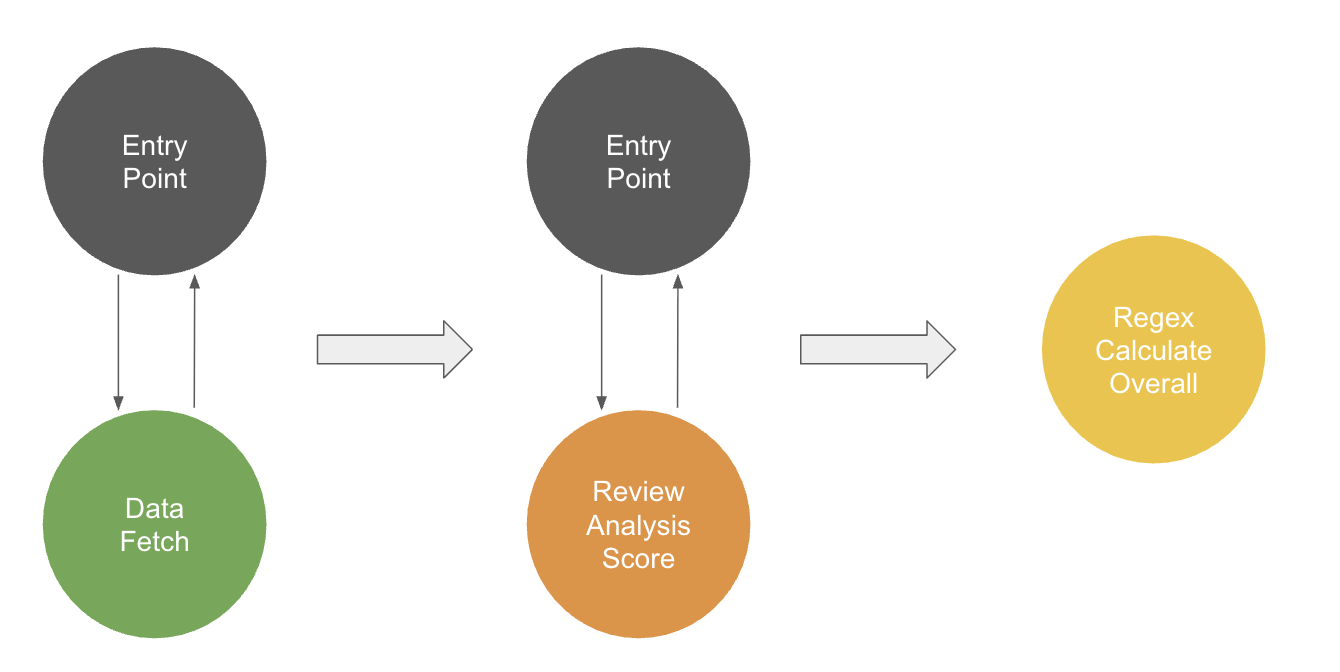
\includegraphics[width=0.8\textwidth]{workflow_diagram.png}
  \caption{Optimized Agents Workflow}
  \label{fig:workflow}
\end{figure}
\newpage

%--------------------------------------------------
\section*{Prompt Design}
\label{sec:prompt}
\begin{itemize}
  \item I discussed the prompt with \textit{Hao Wei Yei} before passing all public test cases; our prompts may therefore be similar.
  \item We originally used the three-agent setup with detailed, step-by-step instructions. Although this method retrieved and scored in a expected way, it failed to show its robustness in multiple rounds.
  \item Runtime logs showed that during review analysis the agent sometimes fetched incomplete reviews, causing scoring errors.
  \item To fix this, we dropped the step-by-step output—likely overloading the attention mechanism—and now score each review immediately after retrieval, so each score relies only on the most recent sentence.
\end{itemize}

\begin{figure}[h!]
    \centering
    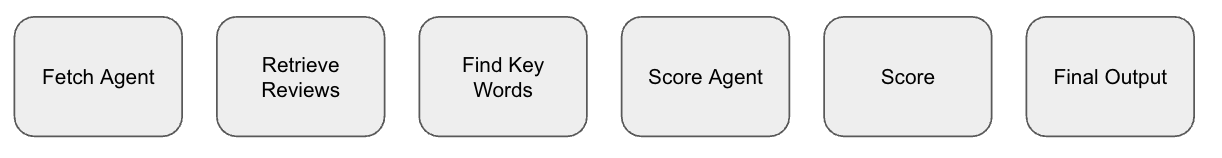
\includegraphics[width=0.8\textwidth]{old_design.png}
    \caption{Original three agents workflow}
    \label{fig:image1}
\end{figure}

\begin{figure}[h!]
    \centering
    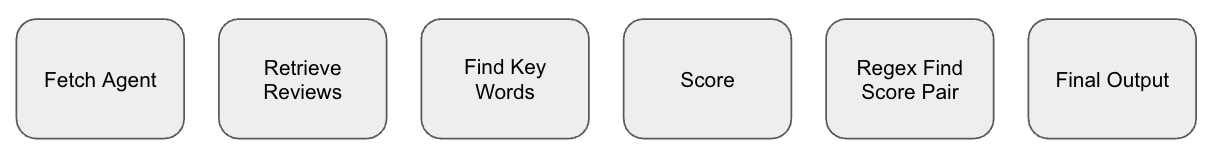
\includegraphics[width=0.8\textwidth]{new_design.png}
    \caption{Our two agents workflow}
    \label{fig:image2}
\end{figure}
%--------------------------------------------------
\section*{Case Analysis: Success and Failure}
\label{sec:cases}
% Compare examples where the model succeeded versus failed.

\subsection*{Success Cases}
% Provide examples and discuss why they were successful.
\begin{itemize}
  \item Example 1: Description and analysis
  \item Example 2: Description and analysis
\end{itemize}

\subsection*{Failure Cases}
% Provide examples where the model did not perform as expected.
Discuss potential causes of failures.
\begin{itemize}
  \item Example 1: Description and error analysis
  \item Example 2: Description and error analysis
\end{itemize}

%--------------------------------------------------
\section*{Conclusion and Key Modifications}
\label{sec:conclusion}
% Summarize lessons learned and outline modifications.
Conclude with the main takeaways and describe any changes you plan to implement to improve performance.

%--------------------------------------------------

\end{document}

